 % !TeX spellcheck = en_US
\documentclass[french]{yLectureNote}

\title{Optique Géométrique}
\subtitle{Niveau 1}
\author{Paulhenry Saux}
\date{\today}
\yLanguage{Français}

\professor{C.Gatel}%christophe.gatel@cemes.fr : section B sillon 7

\usepackage{graphicx}%----pour mettre des images
\usepackage[utf8]{inputenc}%---encodage
\usepackage{geometry}%---pour modifier les tailles et mettre a4paper
%\usepackage{awesomebox}%---pour les boites d'exercices, de pbq et de croquis ---d\'esactiv\'e pour les TP de PC
\usepackage{tikz}%---pour deiffner + d\'ependance de chemfig
\usepackage{tkz-tab}
\usepackage{chemfig}%---pour deiffner formules chimiques
\usepackage{chemformula}%---pour les formules chimiques en \'equation : \ch{...}
\usepackage{tabularx}%---pour dimensionner automatiquement les tableaux avec variable X
\usepackage{awesomebox}%---Pour les boites info, danger et autres
\usepackage{menukeys}%---Pour deiffner les touches de Calculatrice
\usepackage{fancyhdr}%---pour les en-t\^ete personnalis\'ees
\usepackage{blindtext}%---pour les liens
\usepackage{hyperref}%---pour les liens (\`a mettre en dernier)
\usepackage{caption}%---pour la francisation de la l\'egende table vers Tableau
\usepackage{pifont}
\usepackage{array}%---pour les tableaux
\usepackage{lipsum}
\usepackage{yFlatTable}
\usepackage{multicol}
\newcommand{\Lim}[1]{\lim\limits_{\substack{#1}}\:}
\renewcommand{\vec}{\overrightarrow}
\begin{document}
%\titleOne

\setcounter{chapter}{4}
\chapter{Lentilles}
\section{Vergence d'une lentille}
\subsection{Lentille mince formée de 2 dioptres}
Il y a une image intermédiaire entre les 2 dioptres. Il faut utiliser les relations de conjugaison pour chaque dioptre :

On a \(\frac{n}{\bar{S_1A_{i,1}}} - \frac{1}{\bar{S_1A_{o}}} = V_1\) et \(\frac{n}{\bar{S_2A_{i}}} - \frac{1}{\bar{S_2A_{i,1}}} = V_2\). En simplifiant dans le cadre des lentilles minces, $S_1$ et $S_2$ sont confondus et on a \(\frac{1}{\bar{S_2A_{i}}} + \frac{1}{\bar{S_1A_{o}}} = V\)

On obtient finalement la relation de conjugaison des lentilles minces :
\begin{theorem}[Relation de conjugaison des lentilles minces]
\(\frac{1}{\bar{OA_{i}}} - \frac{1}{\bar{OA_{o}}} = V_1+V_2 = V\)
\end{theorem}
\section{Éléments cardinaux d'une lentille}
\warningInfo{Centre optique}{
Le sommet et le centre optique sont confondus.}
\begin{theorem}[Distance focale image/objet]
 La distance focale de l'image est $\frac{1}{V}$. De plus, les distances focales objets et images sont opposées
\end{theorem}

On en déduit que les foyers sont symétriques par rapport à O. Enfin, dans le cas d'une lentielle de vergence positive, $\bar{OF_i} >0$ et $\bar{OF_o} <0$
\section{Construction}
%
% Les graphes indiquent $p_i = \bar{OA_i}$ en fonction de $p_o = \bar{OA_o}$. On a $p_i = \frac{p_o}{1+V_{p_o}}$.
\subsection{Lentille convergente}
La focale image est positive et la focale objet négative.

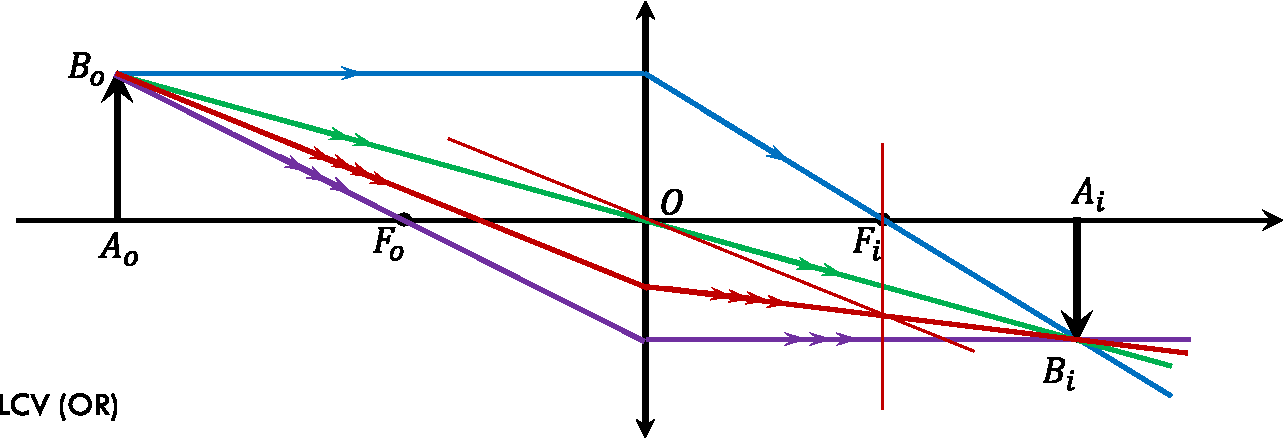
\includegraphics[scale=0.5]{cv-or}

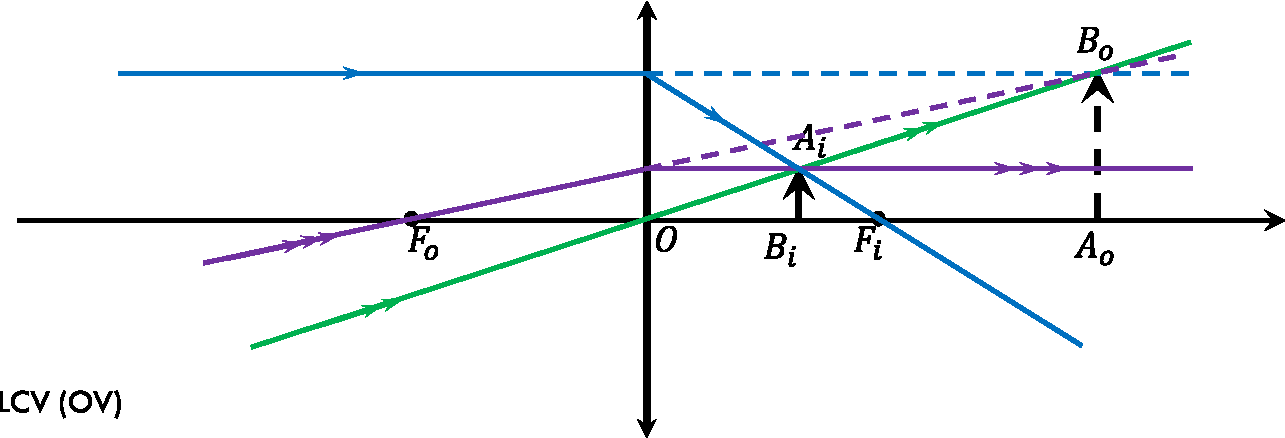
\includegraphics[scale=0.5]{cv-ov}

3 cas possibles :
\begin{itemize}
 \item OR-IR (quand l'objet est avant le foyer objet et avant la lentille)
 \item OR-IV (quand l'objet est après le foyer objet mais avant la lentille)
 \item OV - IR
\end{itemize}
\criticalInfo{Cas impossible}{On ne peut pas avoir une image virtuelle avec un objet virtuel.}

\subsection{Lentille divergente}
La focale image est négative et la focale objet positive.

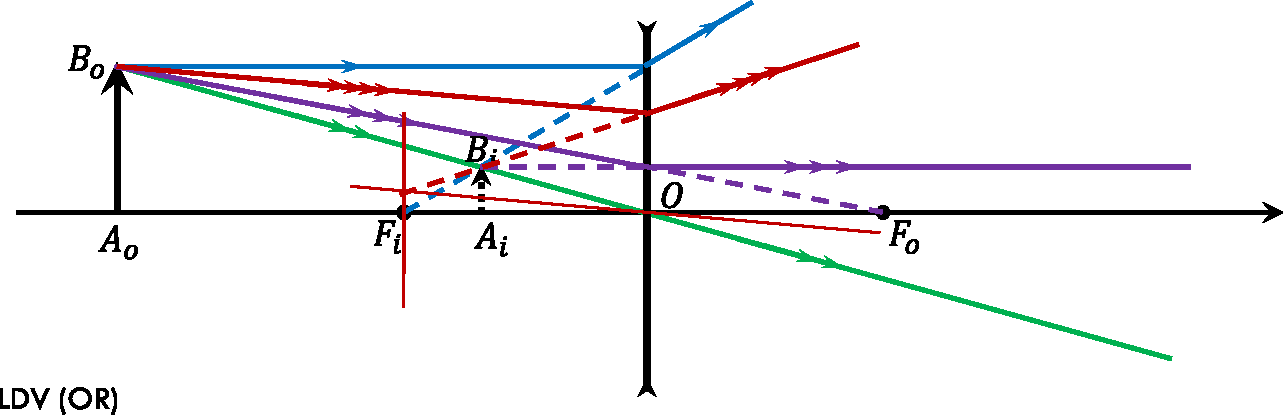
\includegraphics[scale=0.5]{dv-or}

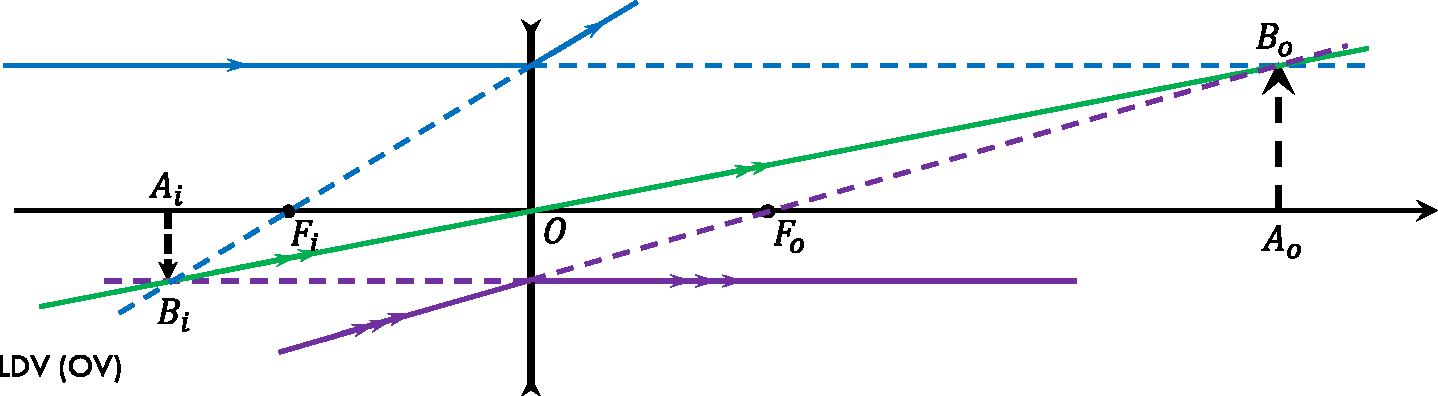
\includegraphics[scale=0.5]{dv-ov}

3 cas possibles :
\begin{itemize}
 \item OR-IV
 \item OV-IR (quand l'objet est avant le foyer objet et après la lentille)
 \item OV - IO  (quand l'objet est après le foyer objet et après la lentille)
\end{itemize}
\criticalInfo{Cas impossible}{On ne peut pas avoir une image réelle avec un objet réel.}
\subsection{Foyers secondaires}
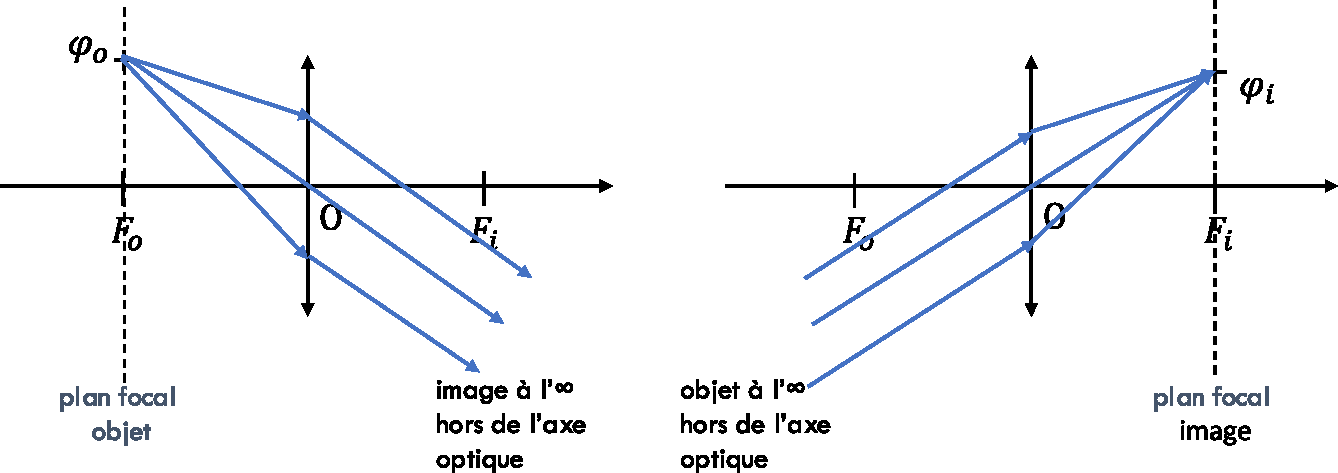
\includegraphics[scale=0.5]{secondaire}
\warningInfo{Foyers secondaires}{Des rayons arrivant parallèlement vont se croiser en un point, se trouvant sur le plan focal image, perpendiculaire à l'axe optique et passant par le foyer image. On a le m\^eme effet pour le foyer objet.}

On utilise les m\^emes règles de construction.
\end{document}

